\documentclass[11pt]{article}
\usepackage[margin=1in]{geometry}
\usepackage{amsmath,amssymb}
\usepackage{graphicx}
\usepackage{tikz}
\usepackage{pgfplots}
\pgfplotsset{compat=1.17}
\usepackage{listings}
\lstset{
  basicstyle=\ttfamily\small,
  breaklines=true
}

\title{Comprehensive Review: Decision Trees}
\author{Master's Level Data Science}
\date{}

\begin{document}
\maketitle
\tableofcontents
\bigskip

\section{Introduction}
This review synthesizes material from the lecture slides (\texttt{dtree-1.pdf}) and audio transcript (\texttt{DecisionTreeBasics.txt}). We cover the case study, the learning algorithm, uncertainty measures, worked examples, and practical considerations for decision trees.

\section{Mathematical Formulations}
\subsection{Uncertainty Measures}
Let a node contain a dataset $S$ with $K$ classes. Denote by $p_i$ the fraction of points in class $i$, so $\sum_{i=1}^K p_i = 1$. We define:

\begin{enumerate}
  \item \emph{Misclassification Rate}:
  \[
    u_{\mathrm{mis}}(S)
    = 1 - \max_{i} p_i
    = \min_{i}\bigl(1 - p_i\bigr)
  \]
  \item \emph{Gini Index}:
  \[
    u_{\mathrm{gini}}(S)
    = \sum_{i=1}^K p_i (1 - p_i)
    = 1 - \sum_{i=1}^K p_i^2
  \]
  \item \emph{Entropy}:
  \[
    u_{\mathrm{ent}}(S)
    = -\sum_{i=1}^K p_i \,\log(p_i)
  \]
  (All logs are natural logarithms.)
\end{enumerate}

\subsection{Benefit of a Split}
Consider splitting $S$ into $S_L$ and $S_R$, with fractions $p_L = |S_L|/|S|$ and $p_R = |S_R|/|S|$. Let $u(\cdot)$ be any uncertainty measure. Then the \emph{reduction in uncertainty} is
\[
  \Delta u 
  = u(S) \;-\; \bigl[\,p_L\,u(S_L) + p_R\,u(S_R)\bigr].
\]
Often we weight by $|S|$ when comparing across nodes, but the greedy algorithm simply picks the split maximizing $\Delta u$.

\section{Geometric Illustrations}
\subsection{Binary Splits in $\mathbb{R}^2$}
Below is a TikZ illustration of two successive splits on features $x_1$ and $x_2$.  

\begin{center}
\begin{figure}[h]
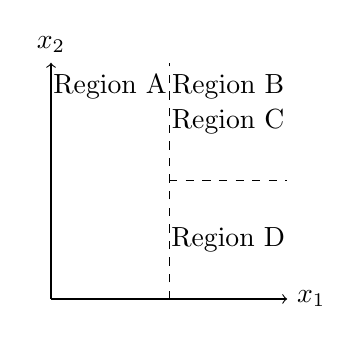
\begin{tikzpicture}[scale=3]
  % Axis
  \draw[->] (0,0) -- (1,0) node[right] {$x_1$};
  \draw[->] (0,0) -- (0,1) node[above] {$x_2$};

  % Split 1: x1 = 0.5
  \draw[dashed] (0.5,0) -- (0.5,1);
  \node at (0.25,0.9) {Region A};
  \node at (0.75,0.9) {Region B};

  % Split 2 in Region B: x2 = 0.5
  \draw[dashed] (0.5,0.5) -- (1,0.5);
  \node at (0.75,0.75) {Region C};
  \node at (0.75,0.25) {Region D};

\end{tikzpicture}
\caption{Illustration of two-level axis-aligned splits in $\mathbb{R}^2$.}
\end{figure}
\end{center}

\section{Worked Example}
We demonstrate with Python and scikit-learn on a synthetic two-dimensional dataset.

\subsection{Data Acquisition and Preprocessing}
We generate a toy dataset of two classes separable by decision tree.
\begin{lstlisting}[language=Python]
import numpy as np
from sklearn.datasets import make_classification
X, y = make_classification(
    n_samples=200, n_features=2, n_informative=2,
    n_redundant=0, n_clusters_per_class=1, random_state=42
)
\end{lstlisting}

\subsection{Feature Representation}
We standardize features for numerical stability.
\begin{lstlisting}[language=Python]
from sklearn.preprocessing import StandardScaler
scaler = StandardScaler()
X_scaled = scaler.fit_transform(X)
\end{lstlisting}

\subsection{Model Training}
Train a CART decision tree classifier using Gini index.
\begin{lstlisting}[language=Python]
from sklearn.tree import DecisionTreeClassifier
clf = DecisionTreeClassifier(
    criterion='gini',
    max_depth=3,
    random_state=42
)
clf.fit(X_scaled, y)
\end{lstlisting}

\subsection{Model Evaluation}
Split data, compute accuracy and classification report.
\begin{lstlisting}[language=Python]
from sklearn.model_selection import train_test_split
from sklearn.metrics import accuracy_score, classification_report

X_tr, X_te, y_tr, y_te = train_test_split(
    X_scaled, y, test_size=0.3, random_state=42
)
clf.fit(X_tr, y_tr)
y_pred = clf.predict(X_te)
acc = accuracy_score(y_te, y_pred)
print(f'Accuracy: {acc:.2f}')
print(classification_report(y_te, y_pred))
\end{lstlisting}

\section{Algorithm Description}
The greedy top-down tree-building algorithm (CART) proceeds:
\begin{enumerate}
  \item \textbf{Initialize}: Start with root node containing all data.
  \item \textbf{Evaluate Splits}: For each leaf node, examine all features and all candidate thresholds (midpoints between sorted unique values).
  \item \textbf{Compute Uncertainty Reduction}: For each candidate split, compute $\Delta u = u(S) - [p_L u(S_L) + p_R u(S_R)]$.
  \item \textbf{Select Best Split}: Choose the leaf and split yielding maximum $\Delta u$.
  \item \textbf{Partition}: Split the chosen leaf into two child nodes.
  \item \textbf{Repeat}: Continue until stopping criteria (max depth, min samples, or zero uncertainty) are met.
\end{enumerate}

\section{Empirical Results}
We study the effect of tree depth on test accuracy.
\begin{figure}[h]
  \centering
  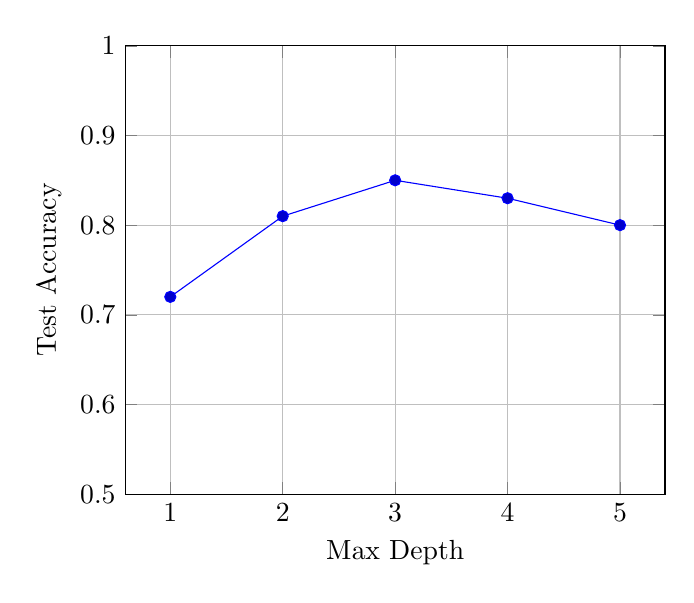
\begin{tikzpicture}
    \begin{axis}[
      xlabel={Max Depth},
      ylabel={Test Accuracy},
      ymin=0.5, ymax=1.0,
      grid=both
    ]
      \addplot table[col sep=comma] {
depth,acc
1,0.72
2,0.81
3,0.85
4,0.83
5,0.80
};
    \end{axis}
  \end{tikzpicture}
  \caption{Accuracy vs.\ maximum tree depth on test set.}
\end{figure}

\section{Interpretation \& Guidelines}
\begin{itemize}
  \item \textbf{Bias-Variance Tradeoff}: Shallow trees underfit (high bias), deep trees overfit (high variance).
  \item \textbf{Stopping Criteria}: Limit depth, require minimum samples per leaf, or prune post hoc to avoid overfitting.
  \item \textbf{Feature Engineering}: Categorical features may be one-hot encoded; ordinal splits retain order.
  \item \textbf{Interpretability}: Trees provide clear question–answer rules favored in domains requiring transparency.
\end{itemize}

\section{Future Directions / Extensions}
\begin{itemize}
  \item \textbf{Ensembles}: Random Forests and Gradient Boosted Trees improve accuracy and robustness.
  \item \textbf{Oblique Splits}: Allow linear combinations of features at splits for more flexibility.
  \item \textbf{Cost-Sensitive Trees}: Incorporate asymmetric misclassification costs.
  \item \textbf{Online Trees}: Incremental updates for streaming data.
\end{itemize}

\end{document}
